\documentclass[11pt,oneside,a4paper]{article}
\usepackage[margin=1.38in]{geometry}
\usepackage{graphicx}
\usepackage{amsmath}
\usepackage{hyperref}
\usepackage{siunitx}
\usepackage[super]{nth}
\usepackage{pgfplots}
\usepackage{filecontents}
\usepackage{booktabs}
\usepackage{indentfirst}
\usepackage{listings}
\lstset{emptylines=1,
        breaklines=true,
        columns=fullflexible,
        keepspaces,}


\graphicspath{ {images/} }

%-------------------------------------------------------------------------------
%	TITLE SECTION
%-------------------------------------------------------------------------------

\newcommand{\horrule}[1]{\rule{\linewidth}{#1}} % Create horizontal rule command with 1 argument of height

\title{
\normalfont \normalsize
\textsc{Sapienza University of Rome} \\ [25pt] % Your university, school and/or department name(s)
\horrule{0.5pt} \\[0.4cm] % Thin top horizontal rule
\LARGE Neural Networks \\ % The assignment title
\large Enriching Word Vectors with Subword Information \\
\horrule{2pt} \\[0.5cm] % Thick bottom horizontal rule
}
\author{Ibis Prevedello} % Your name
\date{\normalsize\today} % Today's date or a custom date

\pgfplotsset{compat=1.15}

\begin{document}

\maketitle




%-------------------------------------------------------------------------------


\section{Introduction}

The goal of this project is to construct and train the fastText algorithm to create a word embedding based on the paper 'Enriching Word Vectors with Subword Information' \cite{Bojanowski_2017}, which was developed by Facebook's AI Research (FAIR) lab.

The dataset used for the training was the EuroSense dataset \cite{eurosense}, which is a multilingual sense-annotated resource in 21 languages, however only the subset of the English language was used for this task.

The training was done using a Google Compute Engine instance running a Tesla K80 GPU.

%-------------------------------------------------------------------------------

\section{fasText}

The algorithm here developed is an extension of the continuous skip-gram model, it differs from skip-gram because it uses subword information, so each  word  is  represented  as  a bag of character n-grams. It means that besides the vector information for each word, there is also a vector information for each subword, and the word is represented by the sum of all these representations.

Let's get one sentence of the dataset as an example. The first step is to remove all the punctuation and convert the text to lowercase, as shown below.

\hfill\break
\begin{lstlisting}
'i', 'do', 'believe', 'that', 'it', 'is', 'vital', 'to', 'minimise', 'the',
'grey', 'areas', 'and', 'emphasise', 'fields', 'for', 'cooperation'
\end{lstlisting}
\hfill\break

In order to present the n-grams, the word 'believe' will be used. For this word, using only n-grams with size three, the n-grams presented below are generated.

\hfill\break
\begin{lstlisting}
'<be', 'bel', 'eli', 'lie', 'iev', 'eve', 've>'
\end{lstlisting}
\hfill\break

Notice that the word starts with the character \lstinline{'<'} and finishes with the character \lstinline{'>'}, therefore the n-gram \lstinline{'lie'} from \lstinline{'believe'} is different from the word \lstinline{'<lie>'}, and they are mapped to different vectors. For the default fastText algorithm it is used n-grams with length varying from 3 to 6 characters, however, for the training, different values were tested.

The use of this n-grams generates another problem, which is the memory limit. There is not enough space in memory to save one vector for each n-gram, therefore a hashing function is necessary to map n-gram to integers in the range 1 to K, where K=2.10\textsuperscript{6}, it means that different n-grams will be mapped to the same vector. The hashing function used is the Fowler-Noll-Vo hashing function (specifically the \lstinline{FNV-1a} variant)\cite{fnv-1a}.
Using the same word \lstinline{believe}, the hash numbers generated for the same n-grams presented before are the following:

\hfill\break
\begin{lstling}
168602, 1819652, 1880439, 1112985, 1135327, 1336773, 1088654
\end{lstling}
\hfill\break

%-------------------------------------------------------------------------------

\section{Network Training}

In order to avoid performing different training by hand, a grid search was implemented, where on each execution a different set of variables were tried from a dictionary containing the name of the parameters and a list of values to be tested. At the end of each training the model was evaluated using the The WordSimilarity-353 Test Collection \cite{wordsimilarity}, and if the correlation was better the model was saved.

The total number of training performed were 29, divided in three stages, 24 training in the first stage, 4 in the second one, and one last training to test the difference when increasing drastically the number of epochs. The parameters tried were the following: window size, embedding size, number of epochs, negative sampling and sizes of n-grams.

%-------------------------------------------------------------------------------

\section{Evaluation}

For the evaluation, as described above, the The WordSimilarity-353 Test Collection \cite{wordsimilarity} was used. This dataset gives a pair of words and a similarity value collect by humans corresponding to the relatedness of the words.

A score is also collected from our model using the cosine similarity considering that the vector representing a single word is the sum of all vector of the word with the n-grams.

In order to check how close the score given by our model is to the human score the Spearman correlation is calculate between the two.

%-------------------------------------------------------------------------------

\section{Results}

Table \ref{tab:first-training} shows the correlation value for the first parameter grid search performed. In this first training the idea was to see how the correlation would behave based on small changes on the parameters. The embedding size and the epoch number was kept constant, and it was possible to notice that the highest correlation achieved was of \textbf{0.308}.

For the second training, table \ref{tab:second-training}, it was kept fixed the minimum and maximum n-gram size and negative count. It was tried to use a window of size 9 because in the previous training the maximum value was obtained with 7, therefore, using a bigger value could maybe lead to a better correlation. The results show that indeed increasing the window size caused a higher correlation, however, a bigger embedding did not present the same effect, achieving a value of \textbf{0.342} for this training.

And, for the last training, table \ref{tab:third-training}, all the parameters were kept the same as the second training, however the idea was to check if increasing the number of epochs to 50 would lead to a significant correlation increase. At this time the correlation value achieved was \textbf{0.359}, showing that the increase was not expressive and possibly this is the best set of parameters using only this dataset.

Figure \ref{fig:pca} shows the Principal Component Analysis (PCA), which executes the dimensionality reduction of 40 important words with the highest number of samples. On this image it is possible to notice that some words that are in fact similar tend to stay close in the graph, for example time and year, committee and council, debate and proposal, Europe and world, and so on. It is also interesting to notice that the words state and states have also similar vectors due to the fact of the n-grams one is a subword of the other.

\begin{table}[]
\centering
\begin{tabular}{rrrrrrr}
\hline
Embedding & Epochs & Min n & Max n & Negative & Window & Correlation \\ \hline
300 & 20 & 2 & 5 & 5 & 3 & 0.257336 \\
300 & 20 & 3 & 5 & 5 & 3 & 0.271176 \\
300 & 20 & 2 & 6 & 5 & 3 & 0.260977 \\
300 & 20 & 3 & 6 & 5 & 3 & 0.272104 \\
300 & 20 & 2 & 5 & 10 & 3 & 0.252319 \\
300 & 20 & 3 & 5 & 10 & 3 & 0.26121 \\
300 & 20 & 2 & 6 & 10 & 3 & 0.264717 \\
300 & 20 & 3 & 6 & 10 & 3 & 0.268816 \\
300 & 20 & 2 & 5 & 5 & 5 & 0.280367 \\
300 & 20 & 3 & 5 & 5 & 5 & 0.29185 \\
300 & 20 & 2 & 6 & 5 & 5 & 0.28114 \\
300 & 20 & 3 & 6 & 5 & 5 & 0.286098 \\
300 & 20 & 2 & 5 & 10 & 5 & 0.269146 \\
300 & 20 & 3 & 5 & 10 & 5 & 0.300445 \\
300 & 20 & 2 & 6 & 10 & 5 & 0.284865 \\
300 & 20 & 3 & 6 & 10 & 5 & 0.296501 \\
300 & 20 & 2 & 5 & 5 & 7 & 0.292673 \\
300 & 20 & 3 & 5 & 5 & 7 & 0.29325 \\
300 & 20 & 2 & 6 & 5 & 7 & 0.301154 \\
\textbf{300} & \textbf{20} & \textbf{3} & \textbf{6} & \textbf{5} & \textbf{7} & \textbf{0.308303} \\
300 & 20 & 2 & 5 & 10 & 7 & 0.28232 \\
300 & 20 & 3 & 5 & 10 & 7 & 0.304186 \\
300 & 20 & 2 & 6 & 10 & 7 & 0.293014 \\
300 & 20 & 3 & 6 & 10 & 7 & 0.306349 \\ \hline
\end{tabular}
\caption{Correlation results for the first stage: it was noticed that there is still room to improve in the window size, 5 being a good value for the negative words and defining 3 and 6 for the minimum and maximum size of the n-grams (the same values suggest by fastText).}
\label{tab:first-training}
\end{table}

\begin{table}[]
\centering
\begin{tabular}{@{}rrrrrrr@{}}
\toprule
Embedding & Epochs & Min n & Max n & Negative & Window & Correlation \\ \midrule
300 & 30 & 3 & 6 & 5 & 7 & 0.339179 \\
\textbf{300} & \textbf{30} & \textbf{3} & \textbf{6} & \textbf{5} & \textbf{9} & \textbf{0.341525} \\
500 & 30 & 3 & 6 & 5 & 7 & 0.316732 \\
500 & 30 & 3 & 6 & 5 & 9 & 0.339169 \\ \bottomrule
\end{tabular}
\caption{Correlation results for the second training: the results were definitely better than the first stage, but still seemed to have some room to improve increasing the number of epochs.}
\label{tab:second-training}
\end{table}

\begin{table}[]
\centering
\begin{tabular}{@{}rrrrrrr@{}}
\toprule
Embedding & Epochs & Min n & Max n & Negative & Window & Correlation \\ \midrule
\textbf{300} & \textbf{50} & \textbf{3} & \textbf{6} & \textbf{5} & \textbf{9} & \textbf{0.359224}
\end{tabular}
\caption{Correlation results for the third training: the correlation improved very little, showing a better result for more epochs but nothing very relevant.}
\label{tab:third-training}
\end{table}

\begin{figure}
  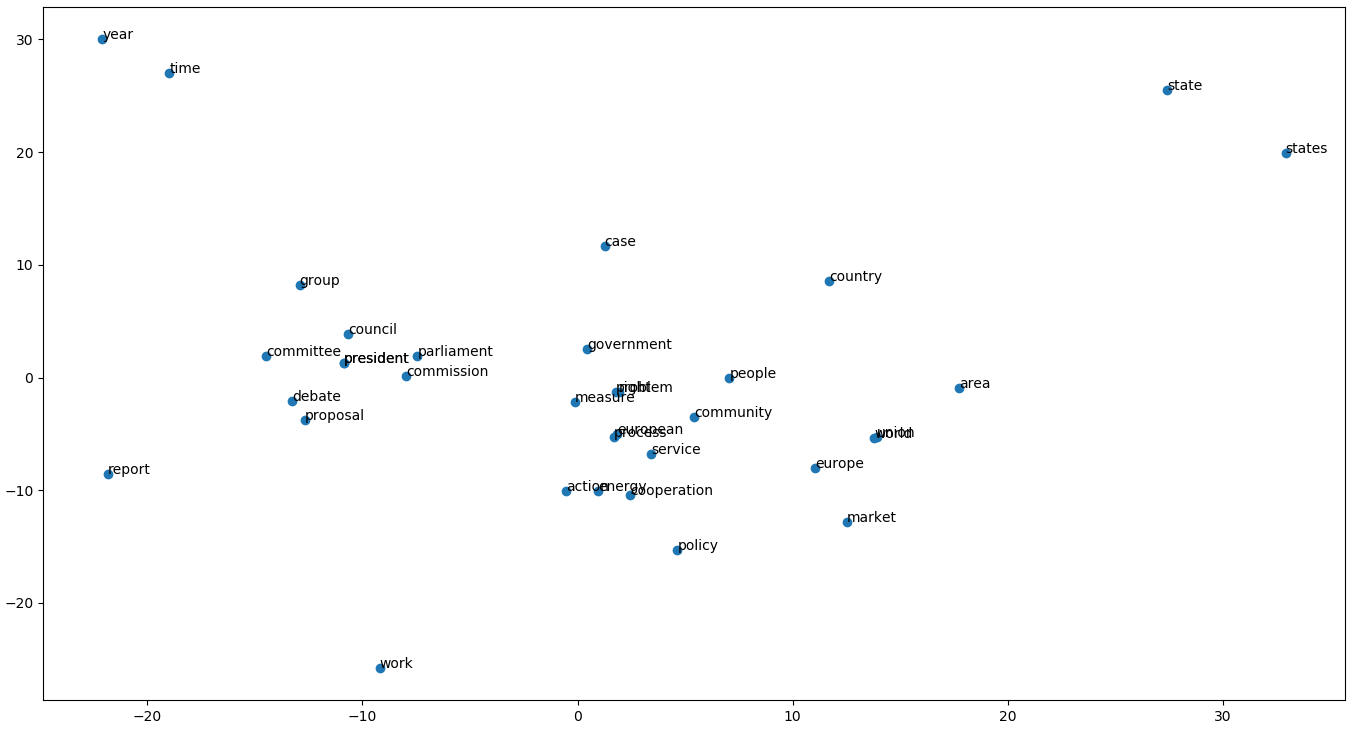
\includegraphics[scale=0.385]{pca.png}
  \centering
  \caption{Dimensionality reduction of 40 words with the highest number of samples.}
  \label{fig:pca}
\end{figure}

%-------------------------------------------------------------------------------

\section{Conclusion}

The goal of this project was to try different set of parameters using fastText algorithm and only one dataset and see what was the best correlation that could be achieved and the effects of these parameters in the model.

It was noticed that this dataset is very limited, it seems to be constructed based on governmental data checking examples from the sentences and the highest frequency words.

After all the tests and parameters set tried, the best correlation achieved was basically \textbf{0.36}, and this is really impressive, because the value reached by me using the same data and a sense embedding structure was \textbf{0.33}, showing the big advantage of using the subword structure for such limited dataset as this.

%-------------------------------------------------------------------------------

\clearpage
\bibliography{bibliography}
\bibliographystyle{ieeetr}

%-------------------------------------------------------------------------------

\end{document}